\documentclass[12pt]{beamer}
\usetheme{Singapore}
\usepackage{mathpazo}
\renewcommand{\rmdefault}{ppl}
\setbeamerfont{title}{family=\rmfamily}
\setbeamerfont{frametitle}{family=\rmfamily}
\usepackage[utf8]{inputenc}
\usefonttheme{professionalfonts} 
\usepackage{amsmath}
\usepackage{amsfonts}
\usepackage{amssymb}
\usepackage{xcolor}
\usepackage{listings}
\usepackage{tikz}
\usetikzlibrary{positioning,fit}

\author{Lai Hao Ran \\ \footnotesize\texttt{hrlai.ecology@gmail.com}}
\title{Basic introduction to\\Bayesian inference}
\date{} 
%\setbeamercovered{transparent} 
\setbeamertemplate{navigation symbols}{} 

\titlegraphic{%
	\centering
	
\includegraphics[height=0.15\textheight]{fig/Marsden-logo-RGB-150.jpg}~%
	\hspace{1cm}
	
\includegraphics[height=0.15\textheight]{fig/University_of_Canterbury_logo.png}~%
	\hspace{1cm}
	
\includegraphics[height=0.15\textheight]{fig/searpp.png}
} 

\lstset{
  basicstyle=\ttfamily\scriptsize,
  breaklines=true,
  showstringspaces=false,
  frame=single,
  backgroundcolor=\color{gray!10},
  literate=
    {~}{{\textasciitilde}}1
    {_}{{\_}}1
    {^}{{\textasciicircum}}1
    {\\}{{\textbackslash}}1
    {|}{{\textbar}}1
    {<}{{\textless}}1
    {>}{{\textgreater}}1
    {=}{{=}}1
}

\newcommand\blfootnote[1]{%
  \begingroup
  \renewcommand\thefootnote{}\footnote{#1}%
  \addtocounter{footnote}{-1}%
  \endgroup
}

\newcommand{\exercise}{%
  \begin{tikzpicture}[remember picture, overlay]
    \node[anchor=north east] at (current page.north east) {
        
\includegraphics[width=2.5cm]{fig/exercise.png}
    };
  \end{tikzpicture}%
}

\begin{document}

\begin{frame}
\titlepage
\end{frame}

\begin{frame}{Today's plan}
Part 1:
\begin{itemize}
\item Three ways to write (and read) a model
\item (Generalised) linear regression
\end{itemize}
\pause
Part 2:
\begin{itemize}
\item Hierarchical / multilevel / mixed-effect model
\item How to make a model go?
\item Interpreting outputs
\end{itemize}
\vfill \pause
We will not explicitly cover:
\begin{itemize}
\item Bayes theorem 
\item Priors
\end{itemize}
\end{frame}

\begin{frame}{Why?}
\pause
How Bayes might reshape our thinking:
\begin{enumerate}[<+->]
\item Understand GLMs better (we will achieve this today)
\item Stop worrying about $p$-values and start to be comfortable with uncertainties
\item See the model as modular; when it fails to converge, understand which part was the culprit
\item It is slower, so you think harder about your model
\item Understand the meaning of each parameter, including the variance term
\item Map my parameters to my questions
\item Your models become \textbf{more purposeful}
\end{enumerate}
\end{frame}

\begin{frame}{Three ways to write (and read) a model}
\begin{Large}
\begin{enumerate}
\item Graphical
\item Code
\item Maths
\end{enumerate}
\end{Large}
\begin{figure}
\centering

\includegraphics[width=0.4\textwidth]{fig/exercise.png}
\end{figure}
\end{frame}

\begin{frame}{The graphical way}
\only<1>{
\begin{center}
The effect of temperature on diversity.
\vfill
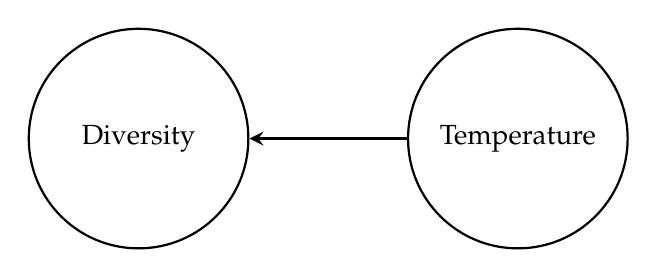
\begin{tikzpicture}[
roundnode/.style={circle, draw, thick, text width=2.5cm, align=center},
]
%Nodes
\node[roundnode] (y) {Diversity};
\node[roundnode] (x) [right=2cm of y] {Temperature};
%Lines
\draw[-stealth, very thick] (x) -- (y);
\end{tikzpicture}
\end{center}
}

\only<2>{
\begin{center}
\begin{tikzpicture}
\draw[-, thick] (0,0) -- node[anchor=north]{Temperature} (5,0);
\draw[-, thick] (0,0) -- node[anchor=south, rotate=90]{Diversity} (0,5);
\end{tikzpicture}

Label axis units \& ticks, add data points, draw regression line
\end{center}
\exercise
}
\end{frame}

\begin{frame}[fragile]{The code way}
\begin{center}
\texttt{lm(Y $\sim$ 1 + X)}
\end{center}
\pause
\begin{lstlisting}
 Family: gaussian  ( identity )
Formula:          y ~ 1 + x

Dispersion estimate for gaussian family (sigma^2): 0.681 

Conditional model:
            Estimate Std. Error z value Pr(>|z|)
(Intercept) -0.03087    0.08296  -0.372    0.710
x            0.03079    0.07936   0.388    0.698
\end{lstlisting}

\end{frame}

\begin{frame}{The maths way}
\only<1-2>{
$$ Y = a + bX + \epsilon $$
}
\only<2>{
\begin{align*}
Y &\sim \text{Normal}(\mu, \sigma_\epsilon) \\
\mu &= a + bX
\end{align*}
}
\only<3->{
$$ Y = \alpha + \beta X + \epsilon $$
}
\only<3->{
\begin{align*}
Y &\sim \text{Normal}(\mu, \sigma_\epsilon) \\
\mu &= \alpha + \beta X
\end{align*}
}
\only<4>{ 
\exercise 
\vfill
Label $\alpha$ and $\beta$ on your graph (try $\mu$, $Y$ and $\sigma$ if you want) 
}
\end{frame}

\begin{frame}{Back to the graphical way}
\begin{center}
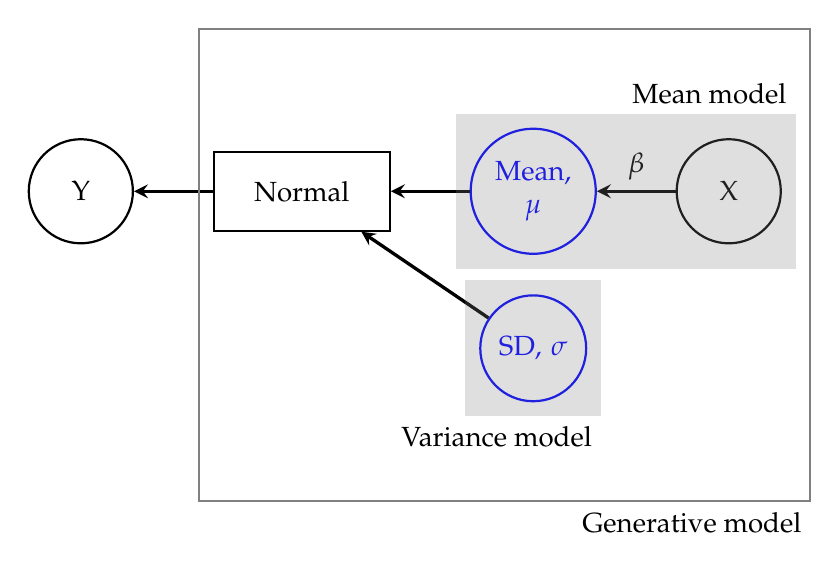
\begin{tikzpicture}[
roundnode/.style={circle, draw, thick, text width=1cm, align=center},
rectnode/.style={rectangle, draw, thick, text width=1cm, align=center},
]
%Nodes
\uncover<1->{ \node[roundnode] (y) {Y}; }
\uncover<3->{ \node[rectnode] (distr) [right=1cm of y, text width=2cm, minimum height=1cm] {Normal}; }
\uncover<2->{ \node[roundnode, blue] (mu) [right=1cm of distr] {Mean, $\mu$}; }
\uncover<1->{ \node[roundnode] (x) [right=1cm of mu] {X}; }
\uncover<4->{ \node[roundnode, blue] (phi) [below=0.5cm of mu] {SD, $\sigma$}; }
%Lines
\uncover<2->{ \draw[-stealth, very thick] (x) -- node[anchor=south]{$\beta$} (mu); }
\uncover<3->{ \draw[-stealth, very thick] (mu) -- (distr); }
\uncover<4->{ \draw[-stealth, very thick] (phi) -- (distr); }
\uncover<5->{ \draw[-stealth, very thick] (distr) -- (y); }
% boxes
\uncover<6->{ 
\node[inner sep=5pt,fill=gray,nearly transparent,fit=(mu) (x)] (meanmod) {};
\node[above left] at (meanmod.north east) {Mean model};
}
\uncover<7->{ 
\node[inner sep=5pt,fill=gray,nearly transparent,fit=(phi)] (varmod) {};
\node[below left] at (varmod.south east) {Variance model};
}
\uncover<8->{ 
\node[inner sep=5pt,draw,gray,thick,minimum height=6cm,fit=(distr) (varmod) (x) (meanmod)] (genmod) {};
\node[below left] at (genmod.south east) {Generative model};
}
\end{tikzpicture} 
\end{center}
\end{frame}

\begin{frame}{What happens if the response is not Normal?}
\begin{center}
Write the model in a general way --- GLMs!
\end{center}
\pause
\begin{align*}
Y &\sim \textcolor{blue}{\text{Distribution}}(\mu,~\phi) \\
\textcolor{blue}{\text{Link-function}}(\mu) &= a + bX
\end{align*}
\pause
\begin{table}
\centering
\begin{tabular}{lll}
\hline
\textcolor{blue}{Distribution} & \textcolor{blue}{Link function} & Typically used for \\
\hline
Normal & Identity & Normal stuff...\\
Binomial & logit / probit & Binary, count with trials...\\
Poisson & log & Counts \\
Negative binomial & log & Counts but clustered \\
Lognormal & log & Skewed continuous \\
Beta & logit & Proportions \\
\hline
\end{tabular}
\end{table}
\end{frame}

\begin{frame}{GLMs are ``generators''}
\begin{figure}
\centering
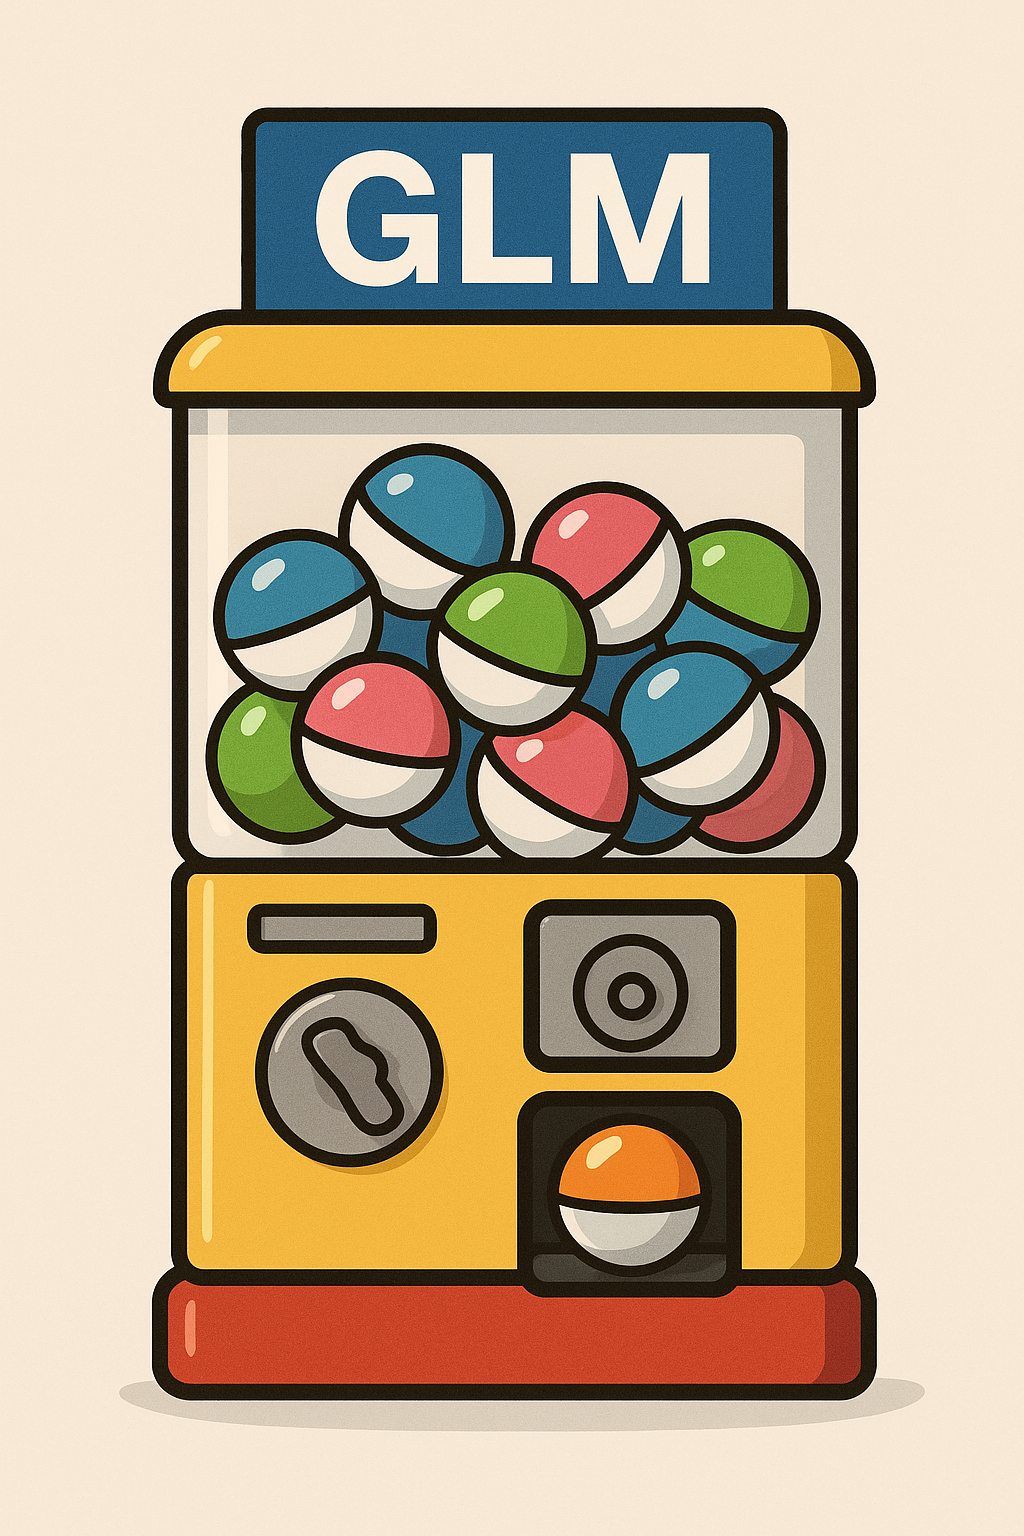
\includegraphics[height=0.8\textheight]{fig/gashapon-glm.png}
\end{figure}
\end{frame}

\begin{frame}{Binomial generator}
\begin{align*}
Y &\sim \textcolor{blue}{\text{Binomial}}(N,~p) \\
\textcolor{blue}{\text{logit}}(p) &= \alpha + \beta X
\end{align*}
\pause
\begin{center}
\begin{tikzpicture}[
roundnode/.style={circle, draw, thick, minimum width=1cm, align=center},
rectnode/.style={rectangle, draw, thick, minimum width=1cm, align=center},
]
%Nodes
\node[roundnode] (y) {Y}; 
\node[rectnode] (distr) [right=1cm of y, text width=2cm, minimum height=1cm] {Binomial}; 
\node[roundnode, blue] (mu) [right=1cm of distr] {Prob.\\logit($p$)}; 
\node[roundnode] (x) [right=1cm of mu] {X}; 
\node[roundnode] (trial) [below=0.5cm of mu] {Trial size\\$N$}; 
\node [below=0.1cm of distr] {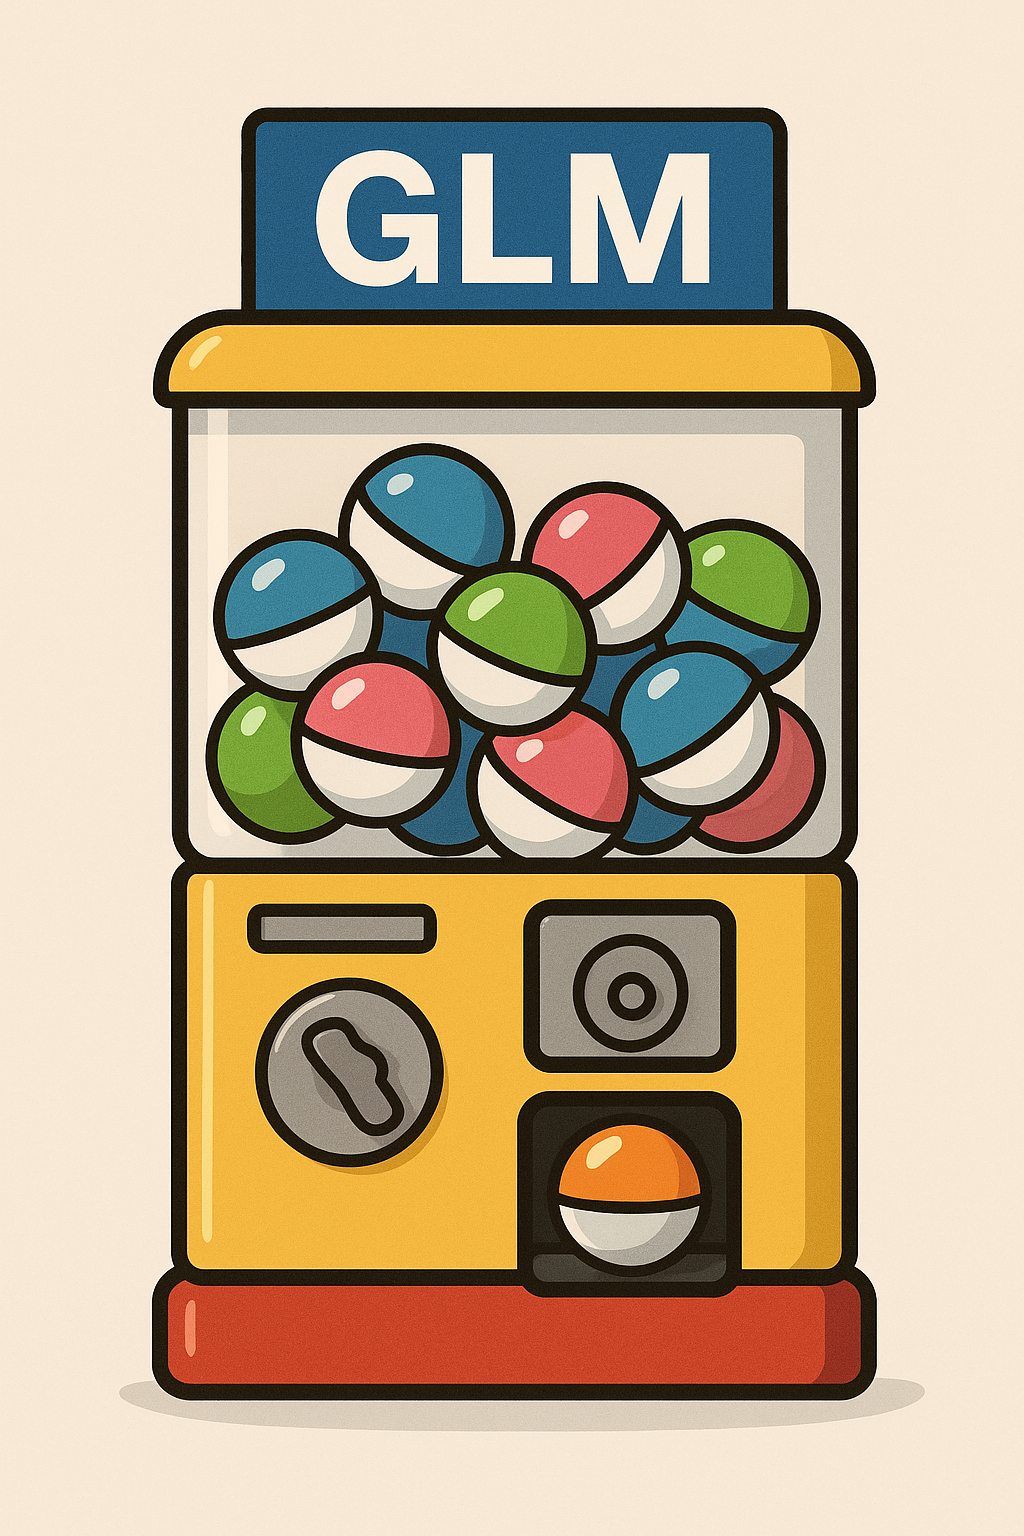
\includegraphics[width=2cm]{fig/gashapon-glm.png}} ;
%Lines
\draw[-stealth, very thick] (x) -- node[anchor=south]{$\beta$} (mu); 
\draw[-stealth, very thick] (mu) -- (distr);
\draw[-stealth, very thick] (trial) -- (distr.south east);
\draw[-stealth, very thick] (distr) -- (y); 
\end{tikzpicture} 
\end{center}
\end{frame}

\begin{frame}{Poisson generator}
\begin{align*}
Y &\sim \textcolor{blue}{\text{Poisson}}(\lambda) \\
\textcolor{blue}{\log}(\lambda) &= \alpha + \beta X
\end{align*}
\pause
\begin{center}
\begin{tikzpicture}[
roundnode/.style={circle, draw, thick, minimum width=1cm, align=center},
rectnode/.style={rectangle, draw, thick, minimum width=1cm, align=center},
]
%Nodes
\node[roundnode] (y) {Y}; 
\node[rectnode] (distr) [right=1cm of y, text width=2cm, minimum height=1cm] {Poisson}; 
\node[roundnode, blue] (mu) [right=1cm of distr] {Rate\\$\log(\lambda)$}; 
\node[roundnode] (x) [right=1cm of mu] {X}; 
\node [below=0.1cm of distr] {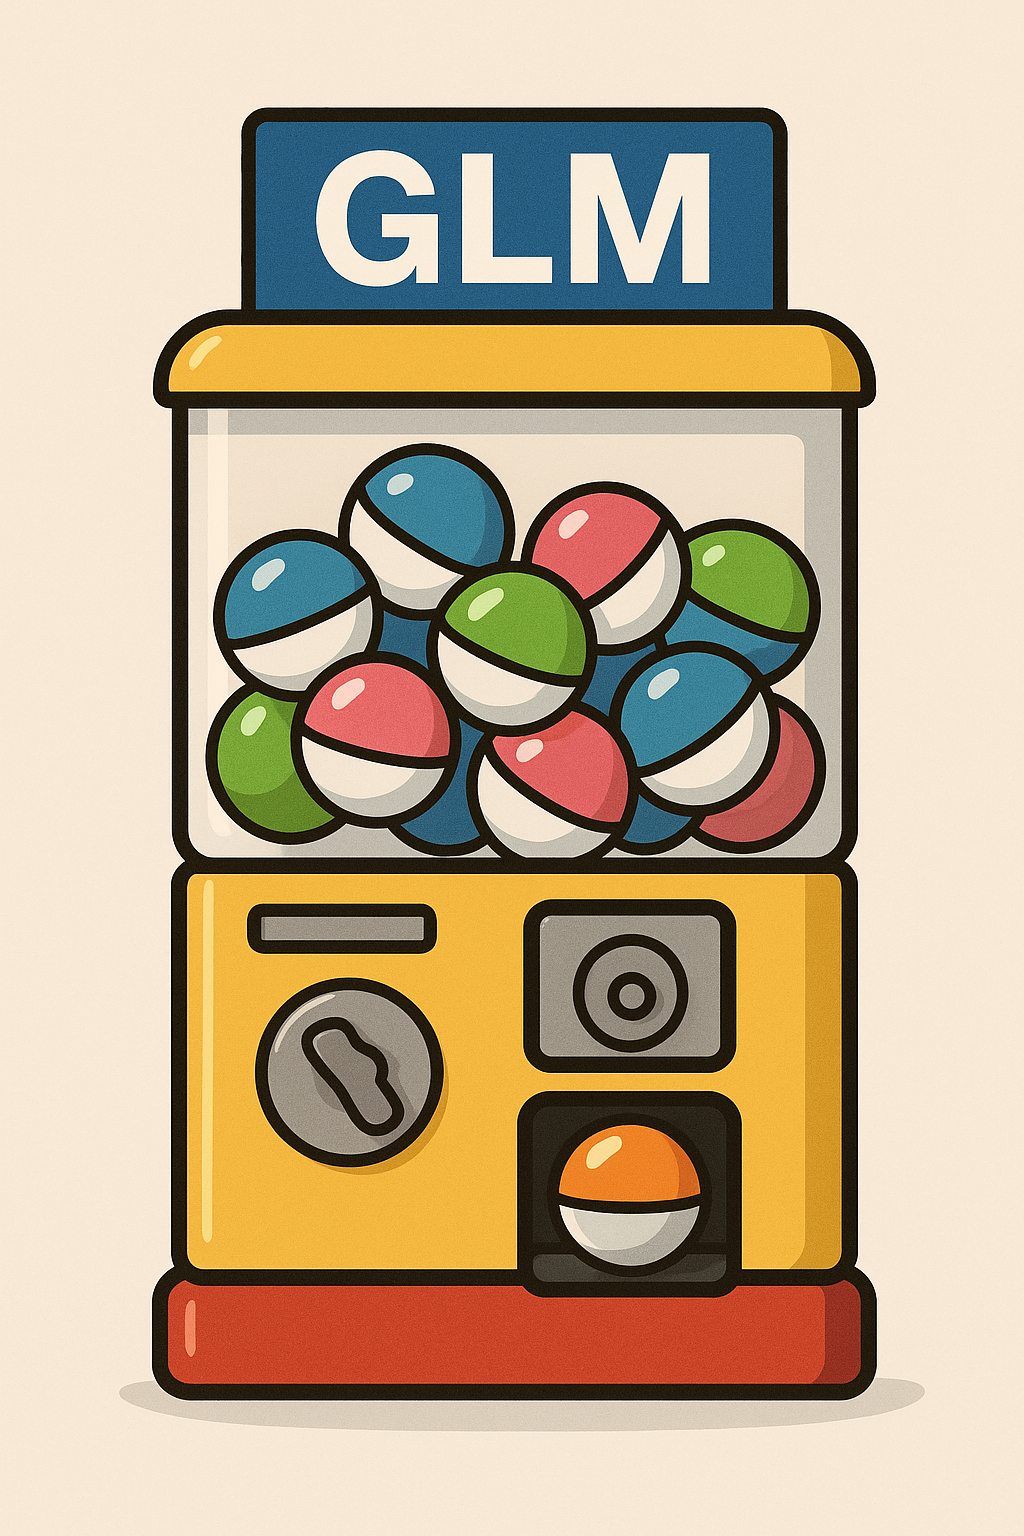
\includegraphics[width=2cm]{fig/gashapon-glm.png}} ;
%Lines
\draw[-stealth, very thick] (x) -- node[anchor=south]{$\beta$} (mu); 
\draw[-stealth, very thick] (mu) -- (distr); 
\draw[-stealth, very thick] (distr) -- (y); 
\end{tikzpicture} 
\end{center}
\end{frame}

\begin{frame}{Negative binomial generator}
\begin{align*}
Y &\sim \textcolor{blue}{\text{Negbinom}}(\mu,~\phi) \\
\textcolor{blue}{\log}(\mu) &= \alpha + \beta X
\end{align*}
\pause
\begin{center}
\begin{tikzpicture}[
roundnode/.style={circle, draw, thick, minimum width=1cm, align=center},
rectnode/.style={rectangle, draw, thick, minimum width=1cm, align=center},
]
%Nodes
\node[roundnode] (y) {Y}; 
\node[rectnode] (distr) [right=1cm of y, text width=2cm, minimum height=1cm] {Negative\\binomial}; 
\node[roundnode, blue] (mu) [right=1cm of distr] {Mean\\$\log(\mu)$}; 
\node[roundnode] (x) [right=1cm of mu] {X}; 
\node[roundnode, blue] (phi) [below=0.5cm of mu] {Dispersion\\$\log(\phi)$}; 
\node [below=0.1cm of distr] {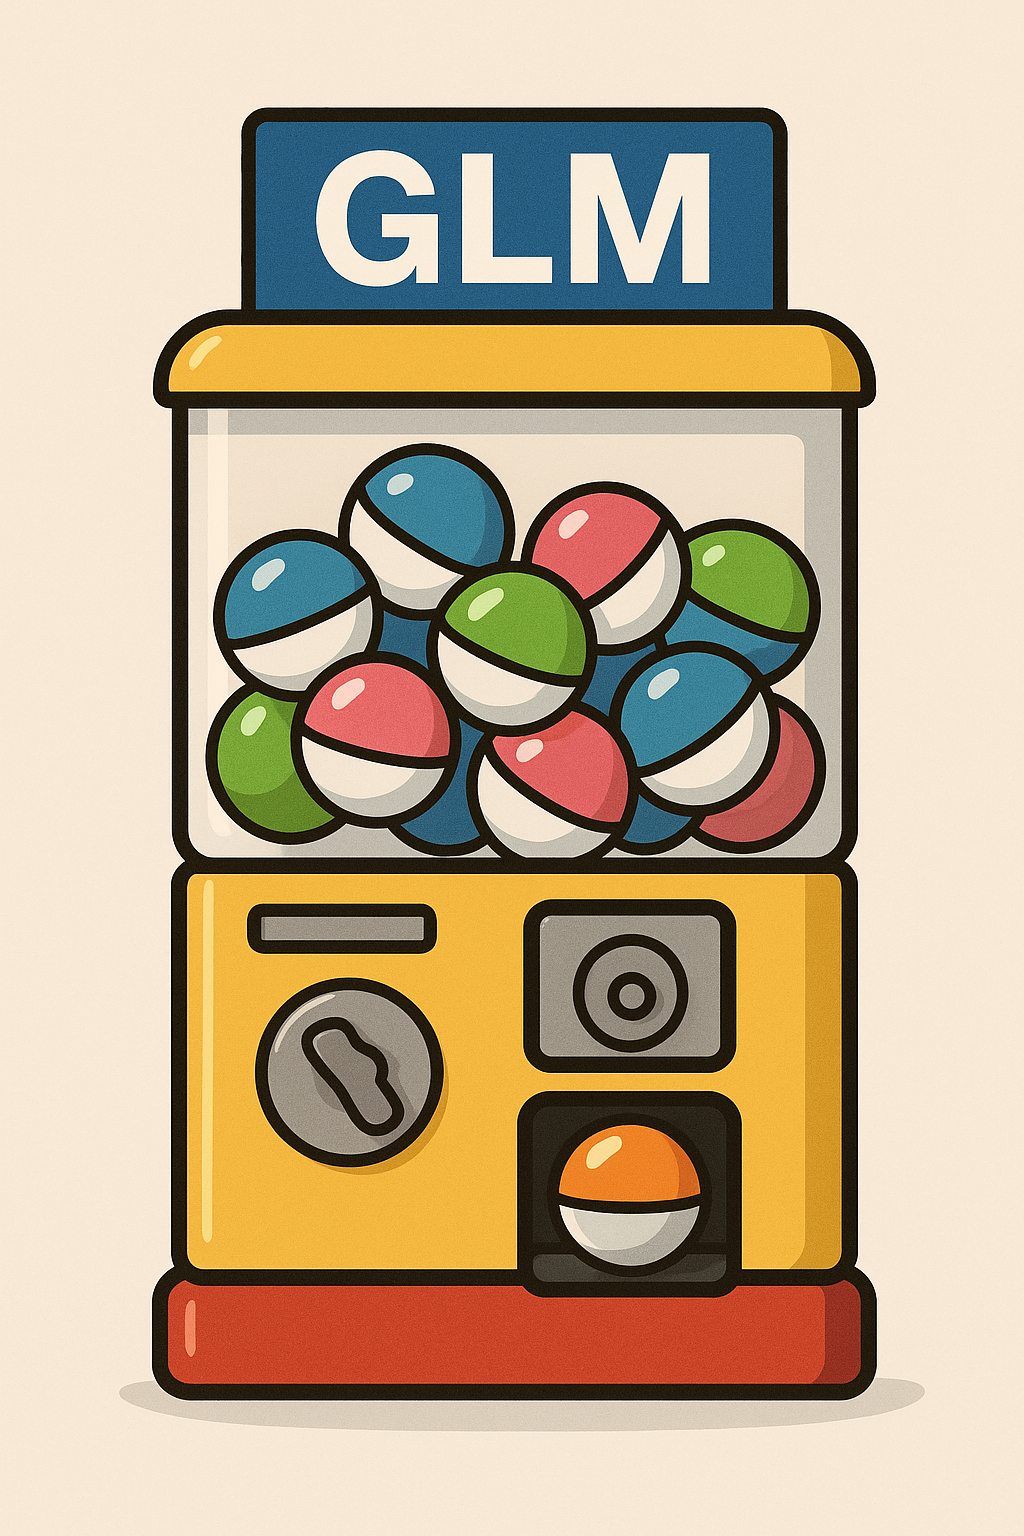
\includegraphics[width=2cm]{fig/gashapon-glm.png}} ;
%Lines
\draw[-stealth, very thick] (x) -- node[anchor=south]{$\beta$} (mu); 
\draw[-stealth, very thick] (mu) -- (distr); 
\draw[-stealth, very thick] (phi) -- (distr.south east);
\draw[-stealth, very thick] (distr) -- (y); 
\end{tikzpicture} 
\end{center}
\end{frame}

\begin{frame}{Back to the code way}
\texttt{glm(Y $\sim$ 1 + X, \textcolor{blue}{family = binomial(link = logit)})}
\vfill
\texttt{glm(Y $\sim$ 1 + X, \textcolor{blue}{family = poisson(link = log)})}
\vfill
\texttt{glm(Y $\sim$ 1 + X, \textcolor{blue}{family = nbinom(link = log)})}
\vfill
\begin{center}
$\vdots$
\end{center}
\end{frame}

\begin{frame}{Combining the ways}
\exercise
\only<1>{
\begin{figure}
\centering
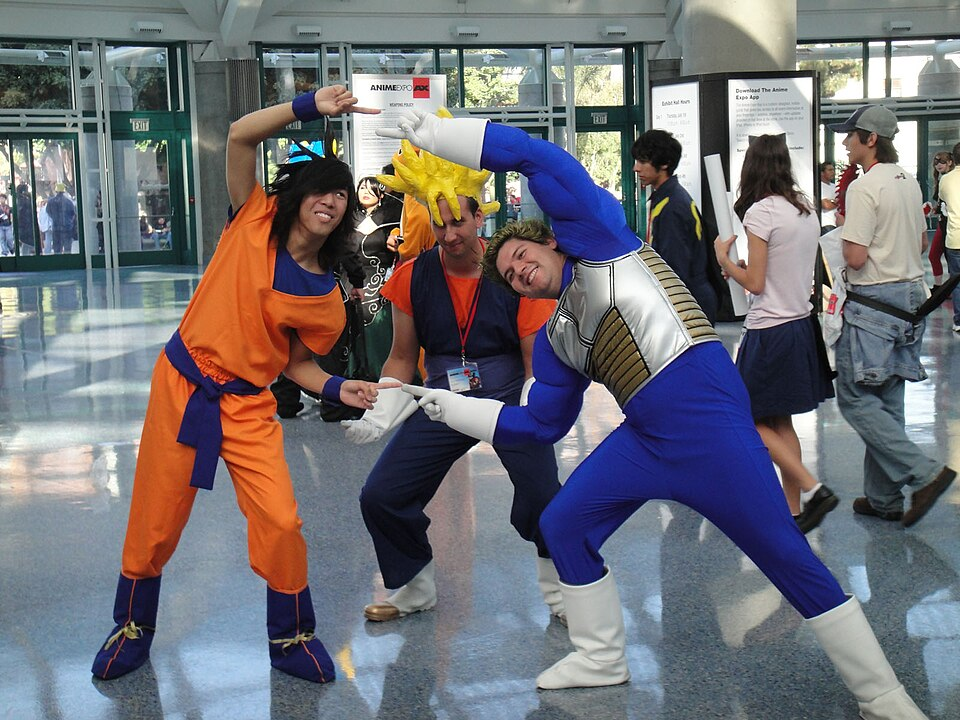
\includegraphics[width=0.7\textwidth]{fig/dragonball-fusion.jpg}
\end{figure}
}
\only<2->{
\begin{enumerate}
\item Express \texttt{Richness $\sim$ 1 + Temperature} mathematically
\item Graph it out; including points, line, and as many labels as you can
\end{enumerate}
}
\uncover<3>{
\begin{center}
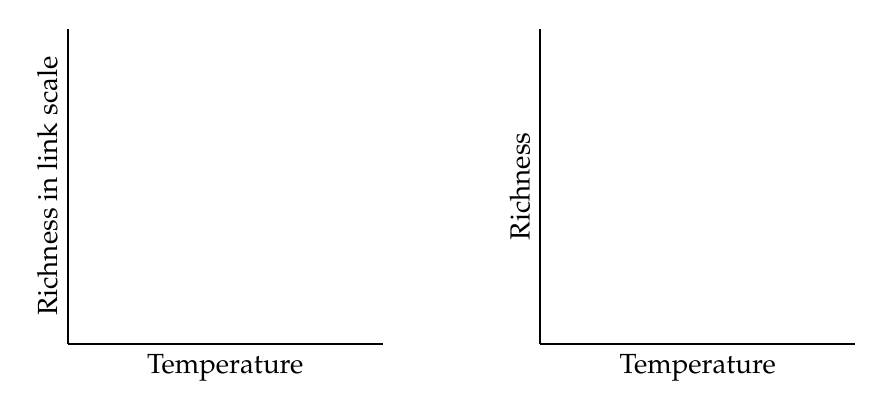
\begin{tikzpicture}
\draw[-, thick] (0,0) -- node[anchor=north]{Temperature} (4,0);
\draw[-, thick] (0,0) -- node[anchor=south, rotate=90]{Richness in link scale} (0,4);
\draw[-, thick] (6,0) -- node[anchor=north]{Temperature} (10,0);
\draw[-, thick] (6,0) -- node[anchor=south, rotate=90]{Richness} (6,4);
\end{tikzpicture}
\end{center}
}
\end{frame}

\begin{frame}{Hang on...where is the Bayesian in this?}
\pause
\begin{center}
In the generative thinking.
\begin{figure}
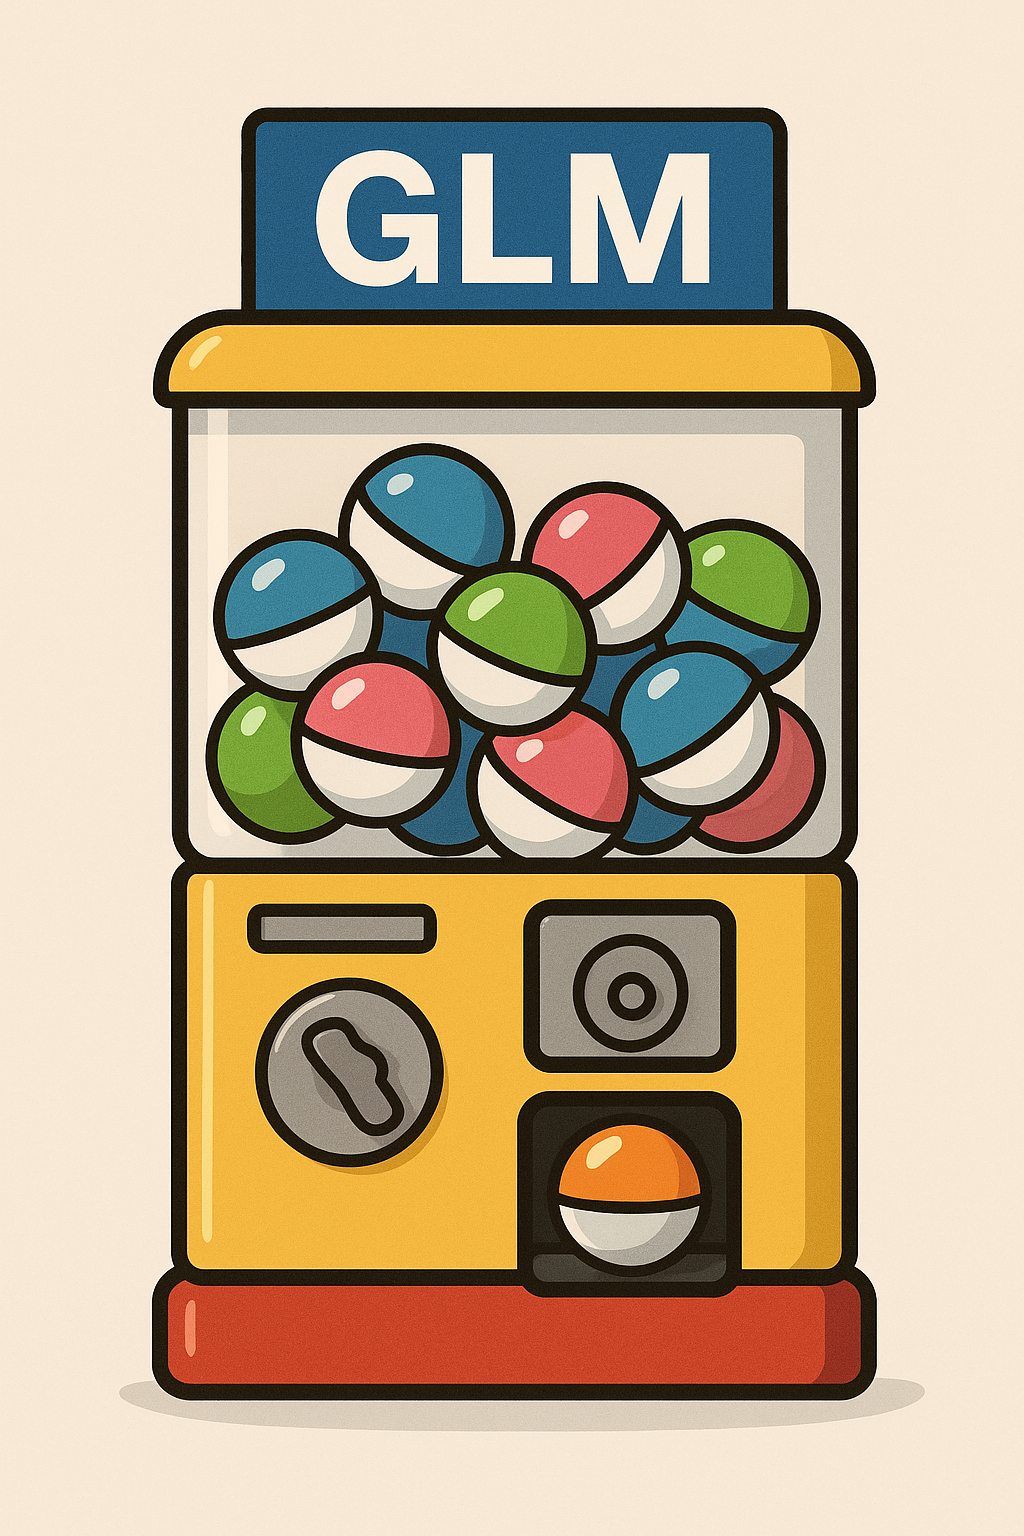
\includegraphics[height=0.5\textheight]{fig/gashapon-glm.png}
\end{figure}
\pause 
Without it, Bayesian inference is no different from frequentist approach --- just another algorithm.
\end{center}
\end{frame}

\begin{frame}{Open session}
\exercise
\begin{center}
Express your analysis to a colleague in a way that is comfortable to \textit{both of you}. 
\end{center}
\end{frame}

\end{document}